\chapter{Phase III - Calcul de taille d'échantillon}

\section{Est-ce important ?}
Dans cette section, on va discuter de l'importance de calculer la taille d'échantillon pour réaliser un essai clinique de phase III.
Un rappel assez bref : \\

\textbf{Phase III}: comparer 2 (ou >2) traitements dans un échantillon de pts\\

\textbf{But}: généraliser nos conclusions à la population

\subsection{Important d’un point de vue méthodologique}
\begin{itemize}
    \item En général, échantillon hétérogène de patients
    \item Une différence observée peut être dû à la chance uniquement
    \item On peut ne pas observer dans notre échantillon une différence existant réellement.
\end{itemize}

\vspace{0.18cm}

\textbf{Les traitements doivent être donnés à un échantillon de patients suffisamment grand pour être représentatif de la population, et de taille adéquate pour contrôler les risques d’erreur de type I et II.}

\subsection{Important pour une utilisation optimale des ressources}
\begin{itemize}
    \item Si trop peu de pts : perte de temps, d’argent et d’efforts, car il est peu probable qu’une telle étude mette au jour des améliorations cliniques
    \item Si trop de pts : gaspillage de temps, d’argent et d’efforts.
\end{itemize}

\subsection{Important d’un point de vue éthique}
\begin{itemize}
    \item Si trop peu de pts : perte de temps, d’argent et d’efforts, car il est peu probable qu’une telle étude mette au jour des améliorations cliniques
    \item Si trop de pts : gaspillage de temps, d’argent et d’efforts.
\end{itemize}

\section{De quoi dépend la taille d’échantillon ?}
\begin{itemize}
    \item Objectif et design de l’essai
    \item Type d’endpoint
    \item Contrôle du risque d’erreur de type I et II (puissance) 
    \item Taille de l’effet traitement que l’on veut mettre en évidence
\end{itemize}

\vspace{0.15cm}

 La taille d’échantillon est déterminée pour obtenir une grande puissance pour détecter un effet du traitement de taille donnée avec un faible risque d’erreur de type I.
 
\subsection{En pratique}
On va se fixer un risque d’erreur de type II ($\beta$), ou de façon équivalente une puissance ($1 − \beta$) pour une alternative prédéfinie et on calcule la taille d’échantillon nécessaire n pour contrôler ce risque à cette valeur.\\

\textbf{Attention aux éléments suivants :}
\begin{itemize}
    \item Si en réalité l’effet du traitement dans la population est plus petit ($< \delta$) alors la puissance sera plus faible que prévu
    \item Si en réalité l’effet du traitement dans la population est plus grand ($> \delta $) alors la puissance sera plus grande que prévu
    \item Avec une taille d’échantillon suffisamment grande même une très petite différence peut être significative
\end{itemize}

\vspace{0.15cm}

\begin{center}
    \textbf{Statistiquement significatif ≠ Cliniquement significatif}
\end{center}

\subsection{Taille de l’effet traitement}
\textbf{Effet traitement cliniquement significatif : }Pour convaincre la communauté médicale de changer leur pratique, il faut démontrer non pas une amélioration, mais bien une amélioration clinique valant la peine de changer la façon de traiter les patients.\\
\textbf{Effet traitement plausible : }L’effet traitement que l’on cherche à mettre en évidence doit être plausible et réaliste.\\

\subsection{Erreur de type I et II}


\section{Comparaison de deux proportions}
\begin{figure}[H]
    \centering
    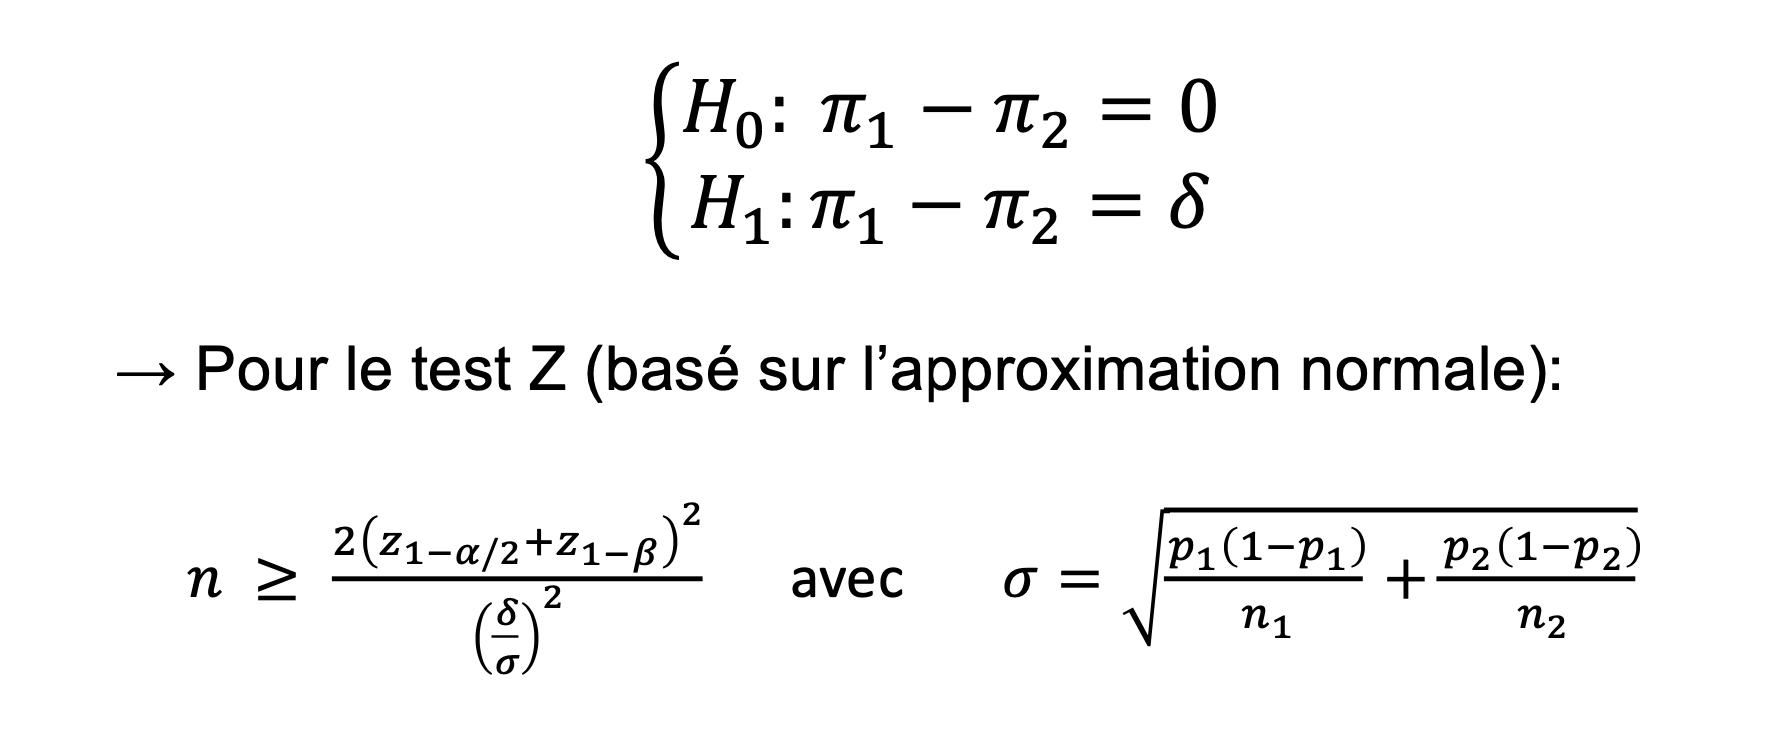
\includegraphics[scale=0.5]{images/comparasion2proportions.png}
    \caption{Comparaison de deux proportions}
    \label{fig:comp2propor}
\end{figure}
La fonction en R : \textbf{power.prop.test}

\section{Comparaison de deux moyennes}
\begin{figure}[H]
    \centering
    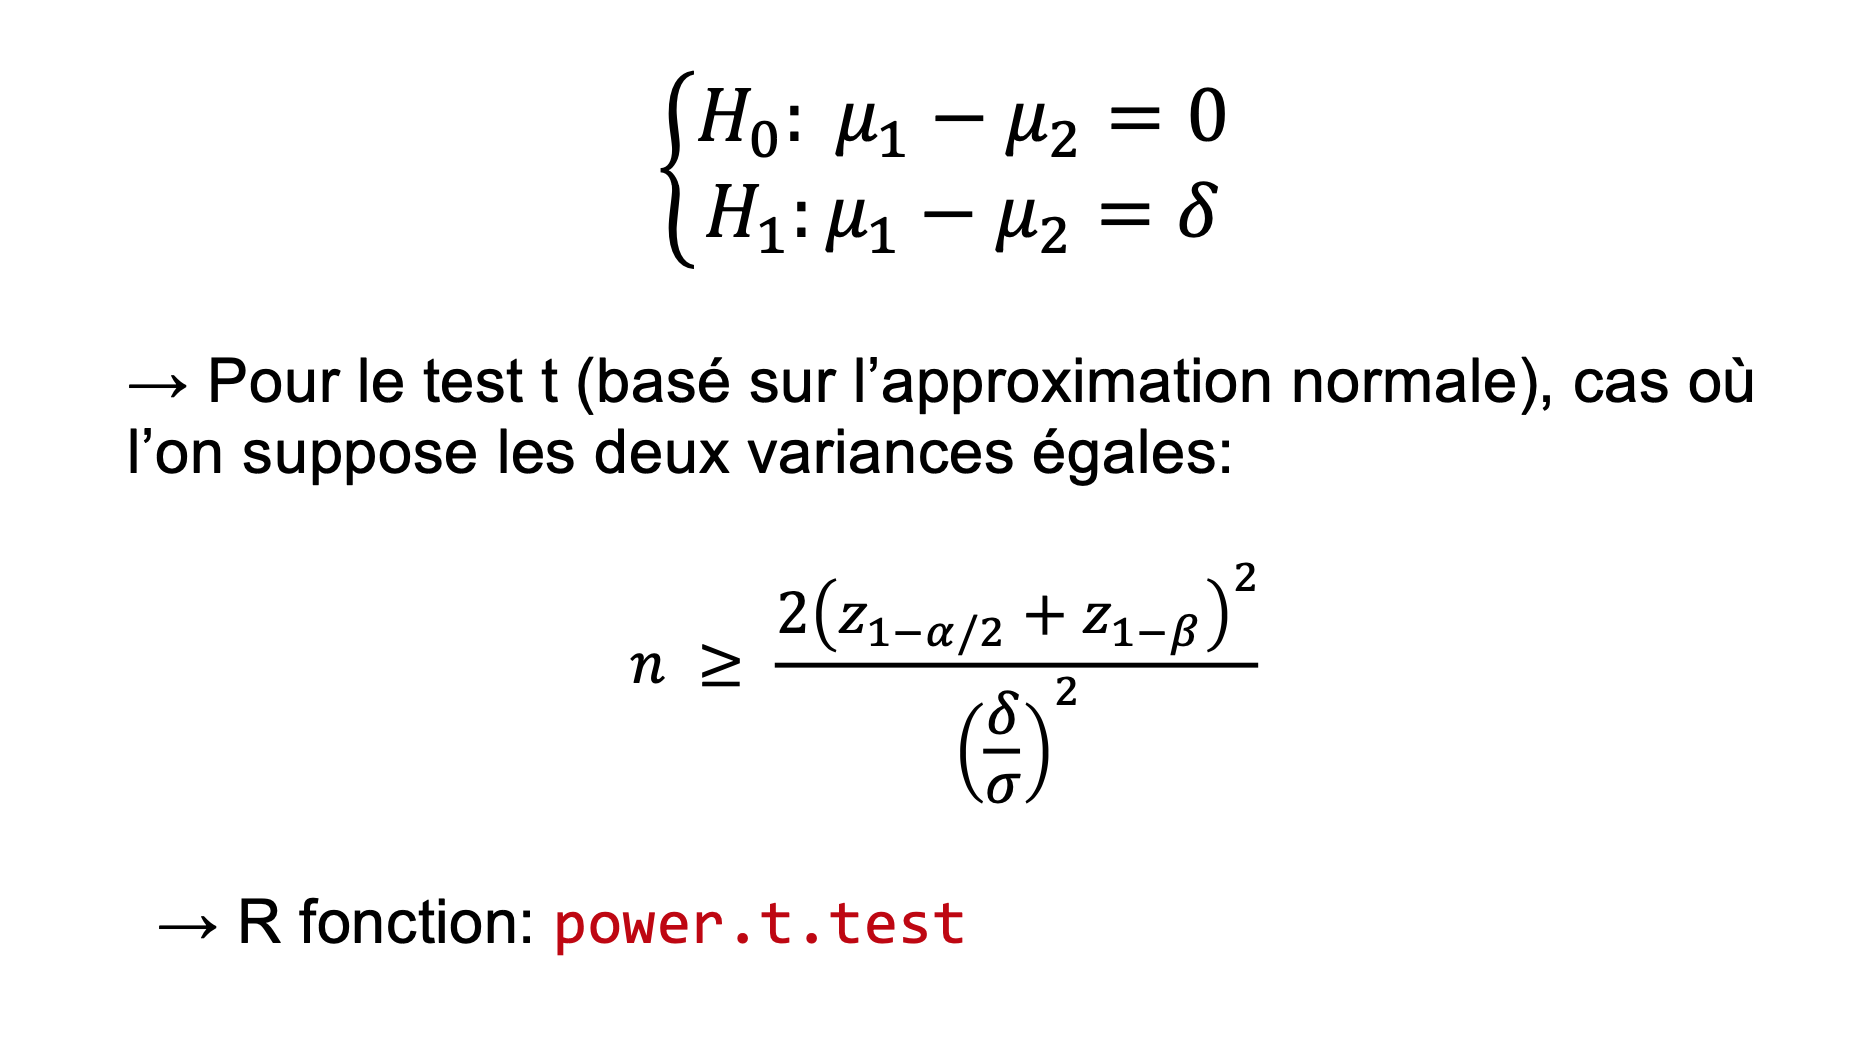
\includegraphics[scale =0.5]{images/comparaison2moyennes.png}
    \caption{Comparaison de deux moyennes}
    \label{fig:comp2moyennes}
\end{figure}
\section{Comparaison de deux courbes de survie}
\begin{figure}[H]
    \centering
    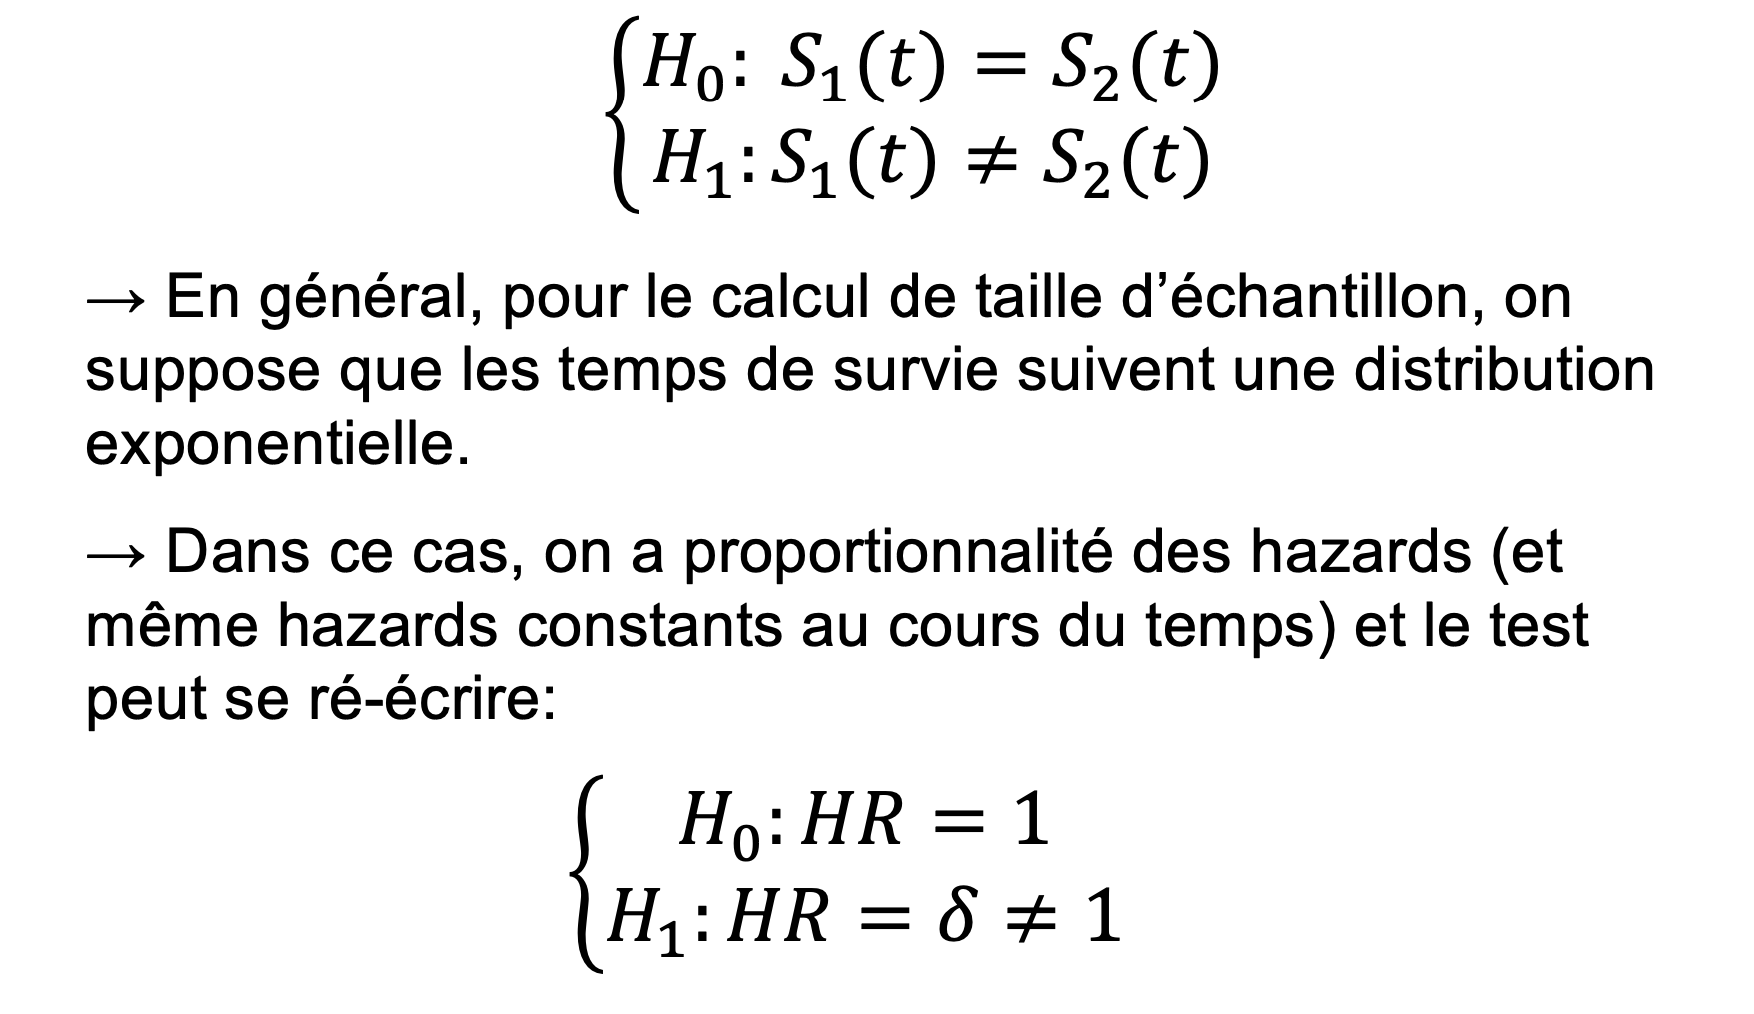
\includegraphics[scale=0.5]{images/comparasion2courbes.png}
    \caption{Comparaison de deux courbes de survies}
    \label{fig:survie}
\end{figure}

\textbf{Dans le cas des données de survie, la puissance n’est pas déterminée par le nombre de patients, mais bien par le nombre d’événements!}
\section{Remarques générales}
Quelques remarques : 
\begin{itemize}
    \item Plusieurs logiciels disponibles:
    \begin{itemize}
        \item Packages/fonctions R, macro/procédure SAS
        \item Packages spécifiques (EAST, Nquery, ...)
    \end{itemize}
\item Parfois plusieurs formules disponibles (solutions approximatives), dans certains cas plus compliqués il n’existe pas de formules ($\Rightarrow simulations$)
 \item Situations plus compliquées si analyses intérimaires (Procédure séquentielle).
\end{itemize}


